\documentclass[fr]{../../../../../../eplexam}
\usepackage{../../../../../../eplunits}
\usepackage{caption}
\usepackage{subcaption}
\usepackage[american]{circuitikz}

\hypertitle{Circuits électroniques}{5}{ELEC}{1530}{2018}{Janvier}
{Martin Braquet \and Olivier Leblanc \and Clément Martin}
{Denis Flandre et Jean-Didier Legat}

\section{}

\begin{enumerate}

\item Question sur le D-FF, dessiner le circuit + commentaire (graphe).
\item Question sur le Multiplexeur et TG. Expliquer le fonctionnement et représenter le multiplexeur optimal à 1 entrée de commande.
\item Considérez le circuit encadré en rouge. Quelle est son utilité? Expliquer comment le polariser afin qu'il fonctionne correctement.

\begin{figure}[h!]
  \begin{center}
    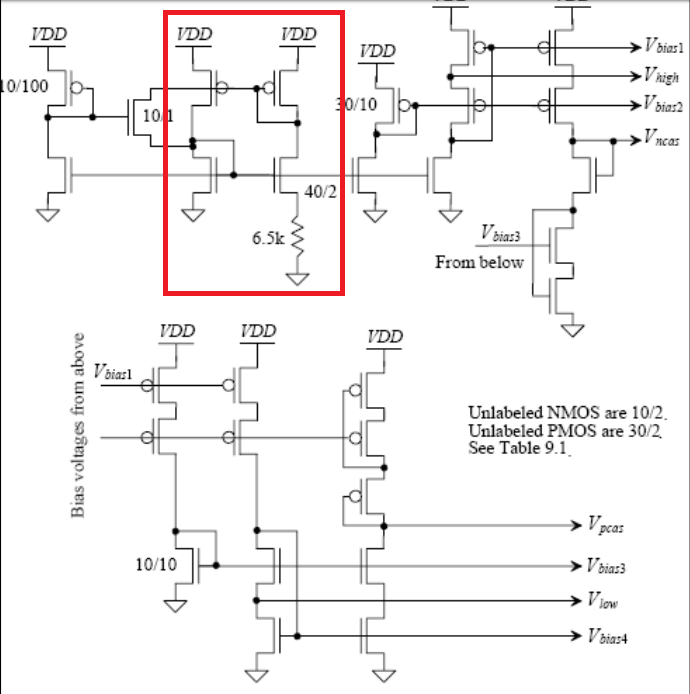
\includegraphics[scale=0.5]{hela} 
    \caption{Schéma du circuit}
  \end{center}
\end{figure}

\item Déterminer le gain du circuit.

\begin{figure}[h!]
  \begin{center}
    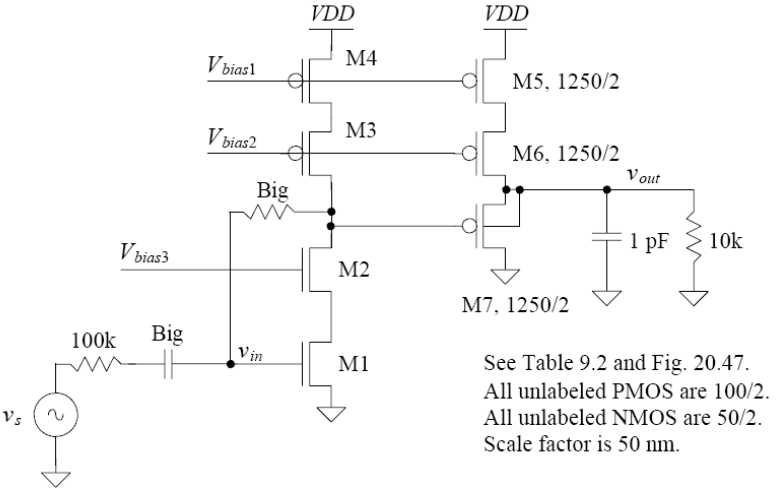
\includegraphics[scale=0.5]{circuit1} 
    \caption{Schéma du circuit}
  \end{center}
\end{figure}

\end{enumerate}

\nosolution

\section{}

\begin{center}
	\begin{circuitikz}
		\draw[thick]
		(2,0) node[npn](npn){}
		(npn.C) -- (2,2.2) node[anchor=south]{VDD}
		(1.8,2.2) -- (2.2,2.2)
		(npn.B) to[short] (0,0)
		(0,2) to[short] (2,2)
		(1,-1) to[short] (2,-1)
		(1,-3) to[short] (2,-3)
		(4,-1) to[short] (6,-1)
		(2,-3) node[sground] {}
		(-4,-2) node[sground] {}
		(4,-3) node[sground] {}
		(6,-3) node[sground] {}
		(0,0) to[R=$R_\mathrm{B}$] (0,2)
		(6,-1) node[above] {$v_{\mathrm{out}}$}
		(-4,0) to[american voltage source,a=$v_{\mathrm{sig}}$,right] (-4,-2)
		(-2,0) to[R=$R_{\mathrm{sig}}$] (-4,0)
		(4,-1) to[R=$R_{\mathrm{L}}$] (4,-3)
		(npn.E) to[R=$R_{\mathrm{E}}$] (2,-3)
		(1,-1) to[I, l_=I] (1,-3)
		(6,-1) to[C=$C_{\mathrm{L}}$] (6,-3)
		(2,-1) to[C=$C_{2}$] (4,-1)
		(0,0) to[C=$C_{1}$] (-2,0);
	\end{circuitikz}
\end{center}

\begin{enumerate}
    \item Définir ce circuit.
    \item Quelles sont les conditions pour que le montage soit correctement polarisé? Donnez les équations mathématiques.
    \item Dessinez le schéma petit-signal. Donnez, dans la bande passante, les résistances d'entrée et de sortie ainsi que LES gains.
    \item Faites une représentation qualitative de la réponse en fréquence, et expliquez comment obtenir un pôle basse fréquence ainsi qu'un pôle haute fréquence. 
\end{enumerate}

\nosolution

\section{}

Données : $C_{ox} = 62.5 \cdot WL \:[\si{aF}], R_n = 34/W \:[\mathrm{k} \Omega], R_p = 68/W \:[\si{k }\Omega]$ 

\begin{figure}[h!]
	\centering
	\begin{subfigure}[t]{0.4\textwidth}
		\centering
		\begin{circuitikz}[ scale=1, american voltages]\draw[thick]
			(0,8) node[pmos](pmos1){}
			(3,8) node[pmos](pmos2){}
			(1,4) node[nmos](nmos3){}
			(-1,4) node[nmos](nmos2){}
			(0,2) node[nmos](nmos1){}
			(0,6) node[nmos](nmos4){}
			(3,6) node[nmos](nmos5){}
			(pmos1.S) --++(0,0) node[vdd]{VDD}
			(pmos2.S) --++(0,0) node[vdd]{VDD}
			(nmos1.S) -- (0,1)
			(0,1) node[sground] {}
			(3,5) node[sground] {}
			(nmos1.G) node[anchor=east] {$CLK$}
			(nmos2.G) node[anchor=east] {$A$}
			(nmos3.G) node[anchor=east] {$B$}
			(nmos4.G) node[anchor=east] {$C$}
			(pmos1.G) node[anchor=east] {$CLK$}
			(1,7) node[anchor=south] {$X$}
			(4,7) node[anchor=east] {$Y$}
			(3,7) -- (3.5,7)
			(3,5) -- (nmos5.S)
			(0,7) -- (2,7)
			(2,6) -- (2,8)
			(nmos5.G) -- (2,6)
			(pmos2.G) -- (2,8)
			(nmos5.D) -- (pmos2.D)
			(nmos4.D) -- (pmos1.D)
			(-1,5) to[short] (1,5)
			(nmos2.D) to[short] (-1,5)
			(nmos3.D) to[short] (1,5)
			(nmos4.S) to[short] (0,5)
			(-1,3) to[short] (1,3)
			(nmos2.S) to[short] (-1,3)
			(nmos3.S) to[short] (1,3)
			(nmos1.D) to[short] (0,3);
			\end{circuitikz}
		\caption{Circuit}
	\end{subfigure}
	%
	\begin{subfigure}[t]{0.4\textwidth}
		\centering
		\begin{circuitikz}[ scale=1, american voltages]\draw[thick]
			(3,8) node[pmos](pmos2){}
			(3,6) node[nmos](nmos5){}
			(pmos2.S) --++(0,0) node[vdd]{VDD}
			(3,7) -- (3.5,7)
			(2,7) -- (1.5,7)
			(nmos5.D) -- (pmos2.D)
			(2,6) -- (2,8)
			(nmos5.G) -- (2,6)
			(pmos2.G) -- (2,8)
			(3,5) -- (nmos5.S)
			(nmos5) node[anchor=west]{10/2}
			(pmos2) node[anchor=west]{20/2}
			(3,5) node[sground] {}
			;
		\end{circuitikz}
		\caption{Inverseur}
	\end{subfigure}
	\caption{Circuits de la question 2.1}
\end{figure}

\begin{enumerate}
    \item Expliquer le fonctionnement du circuit, quel est le type de logique utilisé?
    \item Donner l'équation logique. Vérifier avec une table de vérité.
    \item Dimensionner sur base de l'inverseur unitaire représenté à droite. Justifier succinctement.
    \item Calculer le temps de décharge du nœud de sortie avec $(A, B, C, CLK) = (0, 1, 1, 0) \longrightarrow (0, 1, 1, 1)$ et une capacité de charge de 20fF.
\end{enumerate}

\begin{solution} 

\begin{enumerate}
    \item Logique domino. Principe de fonctionnement : on constate que quand le signal d’horloge est bas (CLK = 0), le noeud X est chargé par le transistor
PMOS du pull-up network, donc la sortie Y = 0 comme $Y = \overline{X}$ . C’est la phase dite de précharge.
Lorsque le signal de clock est haut (CLK = 1), on peut retrouver la fonction logique implémentée par ce
circuit en regardant le pull-down network.
    \item $Y=\overline{X}=C\cdot (A+B)\cdot CLK$
    \item $(W/L)_{n,CLK}=(W/L)_A=(W/L)_B=(W/L)_C=30/2$ et $(W/L)_{p,CLK}=20/2$. Les transistors de l'inverseur entre $X$ et $Y$ sont dimensionnés comme l'inverseur unitaire.
    \item Calculons le temps de décharge de X, puis le temps de charge de Y : 
    \begin{itemize}
        \item Pour $t_{PHL,1}$, nous avons 3 transistors NMOS en série de taille $\frac{30}{2}$ : $N=3$ et $R_n=\frac{34}{15}~[k\Omega]$. Dès lors,
        $$t_{PHL,1} = 3 \cdot 0.7 \cdot C_{load} \cdot R_n + 0.35 \cdot 9 \cdot R_n \cdot C_{oxn}$$
        où $$C_{load}=\frac{3}{2}(C_{oxn,inv}+C_{oxp,inv})+C_{oxp,CLK}=\frac{3}{2} \cdot (10+5) \cdot 62.5\cdot 10^{-18}+10 \cdot 62.5\cdot 10^{-18}=\SI{2.03125}{\femto\farad}$$ et $$C_{oxn}=15\cdot62.5\cdot 10^{-18}=\SI{0.9375}{\femto\farad}$$
        On a donc $t_{PHL,1}=\SI{1.63625}{\pico\second}$.
        \item Pour $t_{PLH,2}$, nous considérons le transistor PMOS car il charge Y. Dès lors, $$t_{PLH,2} = 0.7 \cdot C_{load} \cdot R_p$$ où $$C_{load}=C_L+C_{oxn,inv}+C_{oxp,inv}=20\cdot 10^{-15}+(10+5)\cdot 62.5 \cdot 10^{-18}=\SI{20.9375}{\femto\farad}$$
        On a donc $t_{PLH,2}=\SI{33.22}{\pico\second}$.
    \end{itemize}
    Finalement, $t_{PHL} =t_{PHL,1}+t_{PLH,2} = \SI{34.857}{\pico\second}$.
\end{enumerate}

\end{solution} 

\section{}

\begin{figure}[h!]
	\centering
	\begin{subfigure}[t]{0.3\textwidth}
		\centering
		\begin{circuitikz}\draw[thick]
		(0,2) node[nmos,anchor=source,xscale=-1] (n1){}
		(0,2) node[sground] {}
		(n1.D) to[R=$R$] (0,6)
		(0,6) node[anchor=south]{VDD}
		(2,2) node[nmos,anchor=source] (n2){}
		(2,2) node[sground] {}
		(n1.G) -- (n2.G)
		(2,4.5) to [short,i=$I_{\mathrm{REF}}$] (n2.D)
		(2,7) node {VDD = \SI{5}{V}}
		(2,6.5) node {$R=\SI{50}{k\Omega}$}
		(n1) node[anchor=east] {M1}
		(n2) node[anchor=west] {M2}
		(1,|- n1.G) -- (1,3.5) -- (0,3.5)
		;
		\draw[dashed,thick] (2,4.5) -- (2,5.5);
		\end{circuitikz}
		\caption{}
		\label{a}
	\end{subfigure}
	\begin{subfigure}[t]{0.6\textwidth}
	\centering
	\begin{circuitikz}\draw[thick]
		(0,2) to[I, l=$I_{\mathrm{REF}}$,*-] (0,0)
		(-0.5,2) node[nmos,anchor=source] (n1){}
		(0.5,2) node[nmos,anchor=source,xscale=-1] (n2){}
		(n1.G) node[anchor=east] {$v_{\mathrm{in},1}$}
		(n2.G) node[anchor=west] {$v_{\mathrm{in},2}$}
		(-0.5,2) -- (0.5,2)
		(4.5,0) node[nmos,anchor=source] (n3){}
		(5.5,0) node[nmos,anchor=source,xscale=-1] (n4){}
		(n3.D) node[nmos,anchor=source] (n5){}
		(n4.D) node[nmos,anchor=source,xscale=-1] (n6){}
		(n5.D) node[pmos,anchor=D] (n7){}
		(n6.D) node[pmos,anchor=D,xscale=-1] (n8){}
		(n7.S) node[pmos,anchor=D] (n9){}
		(n8.S) node[pmos,anchor=D,xscale=-1] (n10){}
		(4.5,0) -- (5.5,0)
		(5.5,7) to[short,i=$I_{\mathrm{REF}}$] (n10.S)
		(5.5,7) -- (4.5,7) to[short,i_=$I_{\mathrm{REF}}$] (n9.S)
		(5,7) node[anchor=south]{VDD}
		(5,|- n3.S) node[circ]{}
		(5,0) node[sground] {}
		(n3.G) node[anchor=east] {$v_{\mathrm{bias},4}$}
		(n4.G) node[anchor=west] {$v_{\mathrm{bias},4}$}
		(n5.G) node[anchor=east] {$v_{\mathrm{bias},3}$}
		(n6.G) node[anchor=west] {$v_{\mathrm{bias},3}$}
		(n7.G) node[anchor=east] {$v_{\mathrm{bias},2}$}
		(n8.G) node[anchor=west] {$v_{\mathrm{bias},2}$}
		(n9.G) node[anchor=east] {$v_{\mathrm{bias},1}$}
		(n10.G) node[anchor=west] {$v_{\mathrm{bias},1}$}
		(4.5,4.8) to[short,*-] (-0.5,4.8) -- (n1.D)
		(n2.D) -- (0.5,4.5) to[short,-*] (5.5,4.5)
		(n5.D) -- (4,|-n5.D)
		(4,|-n5.D) node[anchor=east] {$v_{\mathrm{out},+}$}
		(n6.D) -- (6,|-n6.D)
		(6,|-n6.D) node[anchor=west] {$v_{\mathrm{out},-}$};
		\draw[color=red] 
		(7.5,3.3) -- (5.75,3.3)
		(7.5,3.3) node[anchor=west] {$R_{\mathrm{out,p}}$}
		(7.5,2.8) -- (5.75,2.8)
		(7.5,2.8) node[anchor=west] {$R_{\mathrm{out,n}}$};
		\draw[-latex,color=red] (5.75,3.3) -- (5.75,3.5);
		\draw[-latex,color=red] (5.75,2.8) -- (5.75,2.6);
		\draw[dashed,thick] (0,-1) -- (0,0);
	\end{circuitikz}
	\caption{}
	\end{subfigure}
	\caption{Circuits de la question 2.2}
	\label{2.2}
\end{figure}

Données: 
\begin{center}
\begin{tabular}{c c c c}
 $I_{\mathrm{REF}}=\SI{60}{\micro A}$ & $(W/L)_p=45/2$ & $(W/L)_n=15/2$ & $V_{\mathrm{T0,n}}=\SI{0.8}{V}$\\ [2ex]
 $k_n'=\SI{120}{\micro A/V^2}$ & $k_p'=\SI{40}{\micro A/V^2}$ & ${VEA}_n=\SI{50}{V}$ & ${VEA}_p=\SI{33.33}{V}$
\end{tabular}
\end{center}

Note : Les valeurs de réponses ne sont peut-être pas correctes.

\begin{enumerate}
    \item Donnez la fonction du montage présenté à la figure \ref{a}.
    \item Déterminez $(W/L)_1 = (W/L)_2$ dans la figure \ref{a} pour avoir $I_{\mathrm{REF}}=\SI{60}{\micro A}$.
    \item Trouvez toutes les tensions d'overdrive, les transconductances et conductances de sortie de tous les MOS.
    \item Déterminez la borne d'entrée positive du circuit $v_{\mathrm{in,+}}$.
    \item En utilisant le modèle petit signal approprié à chaque fois, trouvez l'expression des résistances de sortie $R_{\mathrm{out,n}}$ et $R_{\mathrm{out,p}}$ ainsi que leur valeur.
    \item En remplaçant les transistors du dessous par la résistance équivalente vue par le noeud de sortie ($R_{\mathrm{out,n}}$), déterminez le gain $v_{\mathrm{out,+}}/v_{\mathrm{in,1}}$. Expression analytique uniquement.
    \item En utilisant la symétrie des branches, que vaut le gain différentiel $A_d = \frac{v_{\mathrm{out,+}}-v_{\mathrm{out,-}}}{v_{\mathrm{in,+}}-v_{\mathrm{in,-}}}$?
    \item Déterminez le pôle $f_L$ si l'on met une capacité de charge de $\SI{20}{\femto \farad}$ (plus sûr de la valeur) à la sortie $v_{\mathrm{out,-}}$.
\end{enumerate}

\begin{solution}

\begin{enumerate}
    \item Il s'agit d'un miroir de courant polarisé par une résistance.
    \item $$(W/L)_1 = (W/L)_2=\frac{2I_{\mathrm{REF}}}{k_n'(VDD-RI_{\mathrm{REF}}-V_{\mathrm{T0,n}})}=\SI{0.6944}{} $$
    \item $V_{OV}=\sqrt{\frac{2I}{k' \left (\frac{W}{L} \right ) }}$
    \begin{table}[h!]
        \centering
        \begin{tabular}{|c|c|c|c|c|c|c|c|c|c|c|}
        \hline
        & $M_{in1}$ & $M_{in2}$ & $M_{bias1}$ & $M_{bias2}$ & $M_{bias3}$ & $M_{bias4}$ &$M_{1}$ & $M_{2}$ \\
        \hline
        $g_m$ [$\si{\micro S}$] & 232.56 & 232.56 & 328.77 & 232.56 & 232.56 & 232.56 & 100 & 100 \\
        \hline
        $g_d$ [$\si{\micro S}$] & 0.6 & 0.6 & 1.8 & 0.9 & 0.6 & 0.6 & 1.2 & 1.2 \\
        \hline
        $V_{OV}$ [V] & 0.258 & 0.258 & 0.365 & 0.258 & 0.258 & 0.258 & 1.2 & 1.2 \\
        \hline
        \end{tabular}
    \end{table}
    \item $v_{\mathrm{in,2}}$ est la borne +. Si on augmente $v_{\mathrm{in,2}}$, le courant traversant ce transistor augmente, donc le courant traversant le transistor dont la grille est $v_{\mathrm{bias,4}}$ diminue car le courant est constant dans le transistor dont la grille est $v_{\mathrm{bias,1}}$. Ainsi, $v_{\mathrm{ DS,bias,4}}$ et $v_{\mathrm{ DS,bias,3}}$ diminuent , donnant finalement une diminution de $v_{\mathrm{out,-}}$. 
    \item $$R_{out,p} = \frac{g_{d1}+g_{d2}+g_{m2}+g_{\mathrm{d,in2}}}{g_{d2}(g_{d1}+g_{\mathrm{d,in2}})} = \SI{109}{\mega \Omega} $$ $$ R_{out,n} = \frac{g_{d3}+g_{d4}+g_{m3}}{g_{d3}g_{d4}} = \SI{649}{\mega \Omega}$$
    \item $$ A_{v+}\overset{\Delta}{=} \frac{v_{\mathrm{out,+}}}{v_{\mathrm{in,1}}}=\frac{-g_{\mathrm{m,in1}}R_{\mathrm{out,n}}}{1+(1+g_{d2}R_{\mathrm{out,n}})\frac{g_{d1}+g_{\mathrm{d,in1}}}{g_{m2}+g_{d2}}} \simeq \frac{-g_{\mathrm{m,in1}}R_{\mathrm{out,n}}}{1+g_{d2}R_{\mathrm{out,n}}\frac{g_{d1}+g_{\mathrm{d,in1}}}{g_{m2}}}$$
    \item $A_{v+}=A_{v-}$ par symétrie.
    $$A_d = \frac{v_{\mathrm{out,+}}-v_{\mathrm{out,-}}}{v_{\mathrm{in,+}}-v_{\mathrm{in,-}}} = \frac{A_{v+}v_{\mathrm{in,1}}-A_{v+}v_{\mathrm{in,2}}}{v_{\mathrm{in,2}}-v_{\mathrm{in,1}}} = -A_{v+} = \frac{g_{\mathrm{m,in1}}R_{\mathrm{out,n}}}{1+(1+g_{d2}R_{\mathrm{out,n}})\frac{g_{d1}+g_{\mathrm{d,in1}}}{g_{m2}+g_{d2}}} = \SI{21513}{V/V}$$
    \item $f_L = \frac{1}{2\pi C_L (R_{out_n} || R_{out_p})} = \SI{973.9}{Hz}$
    
\end{enumerate}

\end{solution}


\end{document}
